% Sorted Binary Tree Example
%
% File:         binary-tree-rotations.tex
% Author:       Bob Walton (walton@acm.org)
% Date:      	Thu Mar 28 14:52:11 EDT 2013
  
\documentclass{minimal}
\usepackage[paperheight=1.2in,paperwidth=4.2in,
            height=1.2in,hoffset=0.05in,
	    voffset=0.05in,left=0in,width=4.2in]{geometry}
\usepackage{color}
\usepackage[usenames]{xcolor}
\usepackage{tikz}
\usepackage{scalefnt}
\usetikzlibrary{arrows}
\begin{document}
\raggedright

\begin{tabular}{l}
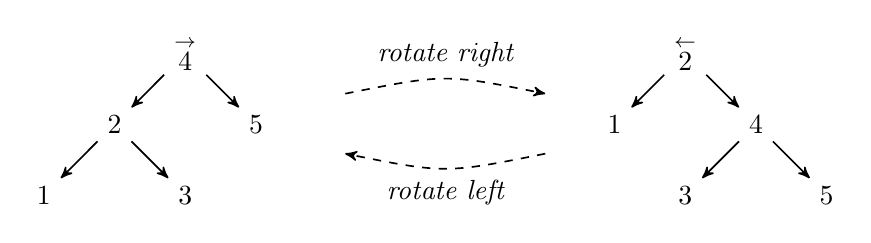
\begin{tikzpicture}[->,>=stealth',auto,
                    node distance=0.5in,semithick,
		    x=1in,y=1in]]

\node[] (ROOT1) at(1,0.8) {$\stackrel{\rightarrow}{\mbox{4}}$};
\node (L1) [below left of=ROOT1] {2};
\node (LL1) [below left of=L1] {1};
\node (LR1) [below right of=L1] {3};
\node (R1) [below right of=ROOT1] {5};

\path (ROOT1) edge (L1) edge (R1)
      (L1) edge (LL1) edge (LR1);

\draw[dashed] (1.8,0.6) .. controls +(0.5,0.1) ..
      node[pos=0.5,above=0.01in,font=\itshape]{rotate right}
      (2.8,0.6);
\draw[dashed] (2.8,0.3) .. controls +(-0.5,-0.1) ..
      node[pos=0.5,below=0.01in,font=\itshape]{rotate left}
      (1.8,0.3);

\node[] (ROOT2) at(3.5,0.8) {$\stackrel{\leftarrow}{\mbox{2}}$};
\node (L2) [below left of=ROOT2] {1};
\node (R2) [below right of=ROOT2] {4};
\node (RL2) [below left of=R2] {3};
\node (RR2) [below right of=R2] {5};

\path (ROOT2) edge (L2) edge (R2)
      (R2) edge (RL2) edge (RR2);
\end{tikzpicture}

\end{tabular}
\end{document}

